% !TEX root = ../MemPod.tex
\section{Results}
\label{sec:Results}

\subsection{Evaluation Framework}
\label{sub:Evaluation}

The goal of our evaluation framework is to quantitatively and qualitatively assess MemPod's capabilities and compare it against state-of-the-art proposed mechanisms. Throughout our evaluation section, we study MemPod's performance running with an eight-core CPU. We extend Ramulator \cite{kim-ramulator} to support flat address space hybrid memories. We model the MemPod architecture,
as well as HMA, THM and CAMEO in our simulation framework. Ramulator enables 
cycle-level memory simulation and includes a simple CPU front-end capable of approximating resource-induced stalls. We chose to evaluate MemPod under a realistic memory configuration consisting of 1GB 3D-stacked HBM \cite{JEDEC-HBM-REVISED} and 8GB of off-chip DDR4-1600. Table \ref{tab:specs} Provides a more detailed description of the simulated system's configuration.

\begin{table}[t]
  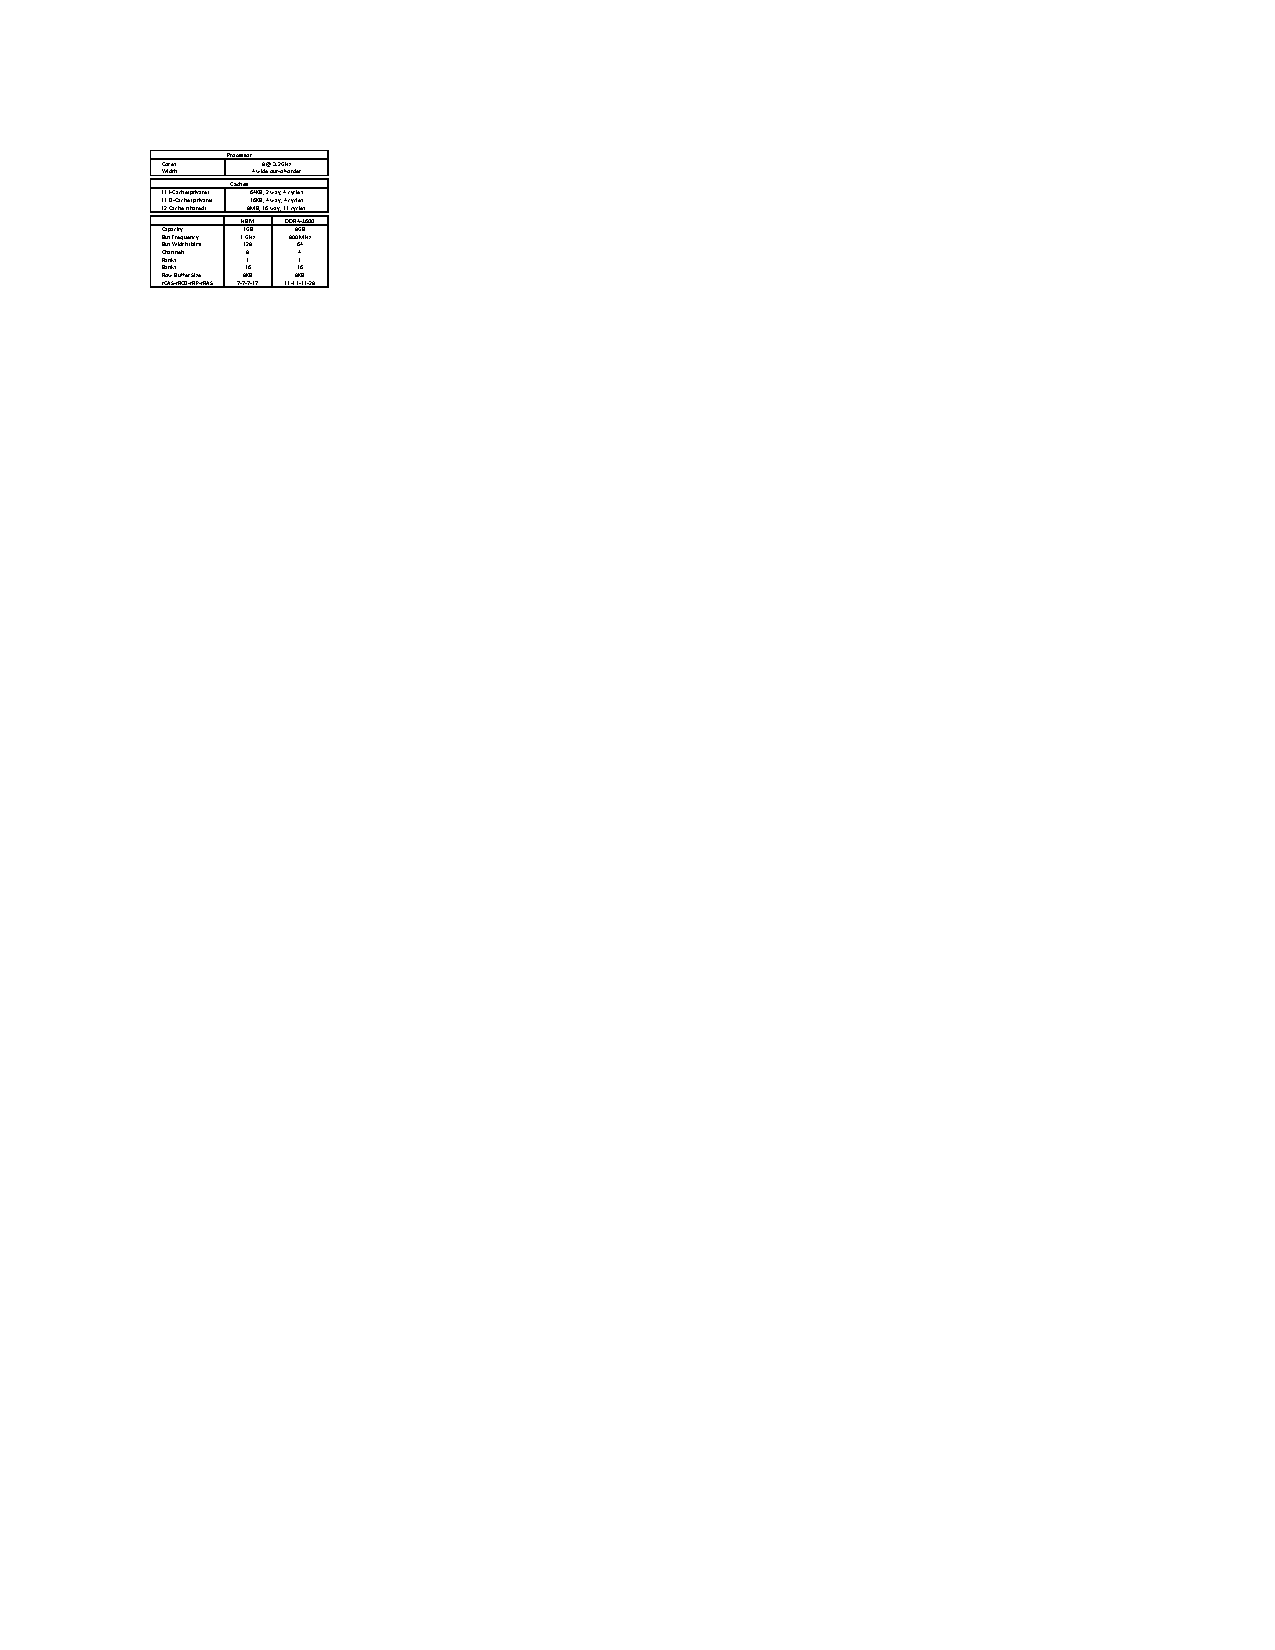
\includegraphics[width=0.46\textwidth]{figures/specs_table.pdf}
  \caption{Experimental framework configuration}
  \label{tab:specs}
\end{table}

\subsection{Experimental Methodology}
\label{sub:Experimental}

We use benchmarks from the SPEC2006 suite \cite{spec} as our workloads. Using Sniper \cite{sniper}, we recorded memory request traces while simultaneously executing 8 benchmarks on a simulated 8-core CPU. We then feed these multi-programmed memory traces into Ramulator, executing all workloads to completion. Our complete set of workloads consists of 15 ``homogeneous'' workloads, where 8 copies of the same benchmark are run in parallel (we simply refer to these workloads by the benchmark's name in later results), as well as 12 workloads featuring a random mix of 8 benchmarks each (referred to as mix1-12). Each benchmark was executed and traced under its reference input. When running homogeneous workloads, Sniper ensures that memory pages are not shared between workloads. A breakdown of the mixed workloads is shown in Table \ref{tab:workloads}.

\remark {A.P.: I'm trying to point out that same benchmarks send memory requests to different pages.}

\remark{I guarantee reviewers are going to ask -- when running 8 copies, 
did you use 8 unique inputs?}

We also extended Ramulator with cacheing for the activity tracking and/or remap tables depending on the simulated mechanism. Cache misses inject memory requests into the stream of requests fed by our trace files to retrieve the missing information. No priority is given to these cache miss requests over regular requests. When caches for hybrid memory management techniques are disabled, the simulator assumes that any information needed by any mechanism exists on chip and is accessible without any delay. The migration process was implemented in detail as well. In order to read an entire 2KB DRAM page from memory, 32 read requests need to be sent for each of the two migration candidates and then another set of 32 requests for each of the two write-backs.

As we use Ramulator with recorded traces, we chose to report Average Main Memory Access Time (AMMAT) in our results. Even though Ramulator has the ability to approximate IPC with a simple CPU model, 
AMMAT is computed with much greater fidelity with this tool, as it models the memory system in great detail. AMMAT is the average time spent accessing and waiting for main memory by each request (lower is better). Due to space limitations we are not able to show results for individual workloads in most of the graphs in this paper. In those graphs, we only present the average of all mixed workloads, average of all homogeneous workloads, and overall average.

In our AMMAT experiments, we typically introduce additional accesses to the
system (migrations, bookkeeping cache misses).  The overhead of the additional
misses is accounted to the total memory stall time, but the total memory 
stall time is divided by the number of original LLC misses (main memory requests) captured in our traces
-- that is, the denominator in our AMMAT equation does not change between
experiments and equals the number of requests in our trace file.

\begin{table}
  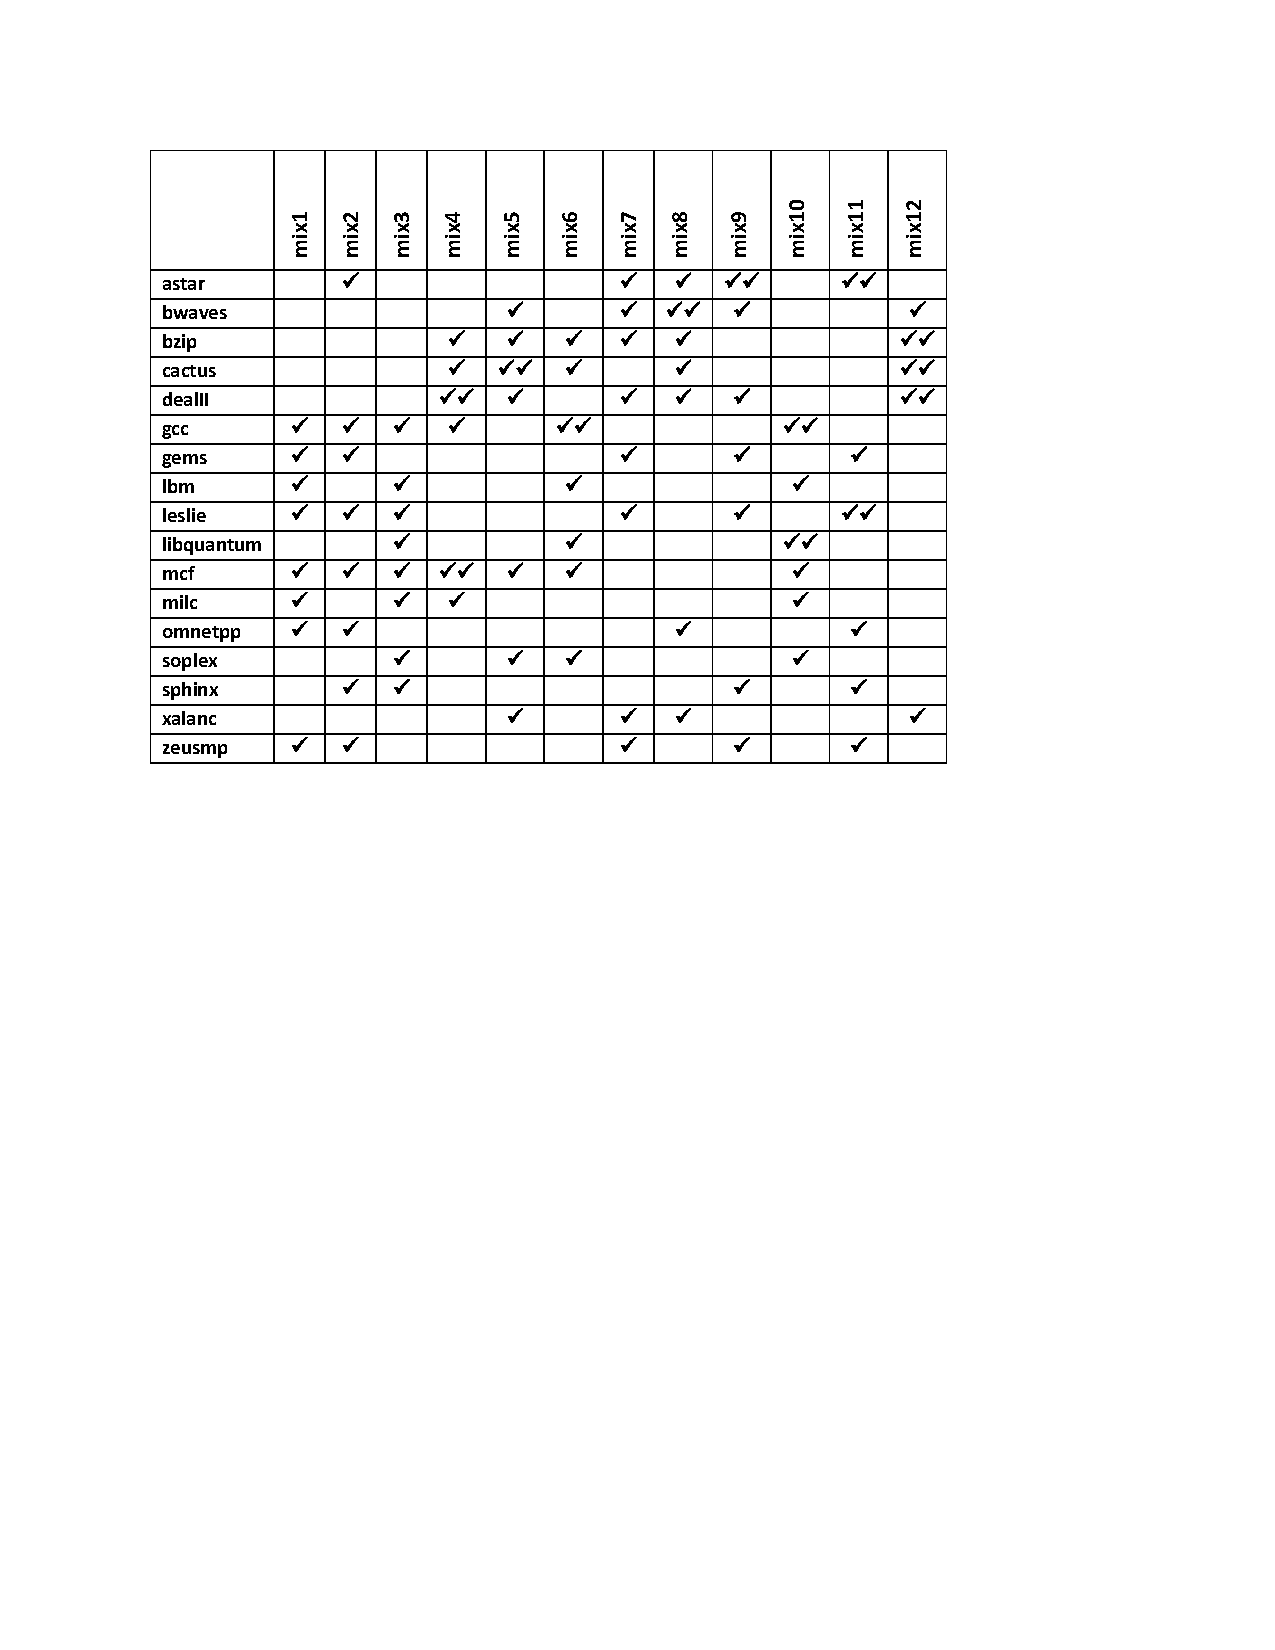
\includegraphics[width=0.46\textwidth]{figures/workloads_checkmarks.pdf}
  \caption{Mixed workloads description}
  \label{tab:workloads}
\end{table}

\subsection{Simulation Results}
\label{sub:SimResults}

\subsubsection{Page Tracking and Migration Design Space}

MemPod's activity tracking overhead and migration traffic is impacted by
the number and size of the MEA counters, as well as the epoch (interval) 
size over
which the counters accumulate.  We examine each of these design space
parameters in this section.
The number of MEA counters dictates the highest possible number of 
migrations that can be performed at each interval by each Pod, while the epoch length will determine MemPod's ability to better adapt to phase changes in a workload. Furthermore, a small number of counters favors less aggressive
migration at each interval boundary.
% temporal locality more than a larger number of counters. 
The size of each MEA counter sacrifices accuracy when smaller counters are 
used 
but can also save space on the chip.  Smaller counters also sacrifice
previous-interval counter accuracy for recency, as it makes it easier to
replace a counter for a previously hot page no longer being accessed.

We first identify the optimal number of counters and epoch length by running a series of experiments. We executed all combinations of epoch length and number of counters pairs with epoch lengths of 25-500us.
We also exponentially increase the number of MEA counters per pod from 16 to 512. In order to minimize the impact of other factors, we execute this experiment with 16 bits per counter and remap table caches disabled. 

\begin{figure}[h]
	\centering
  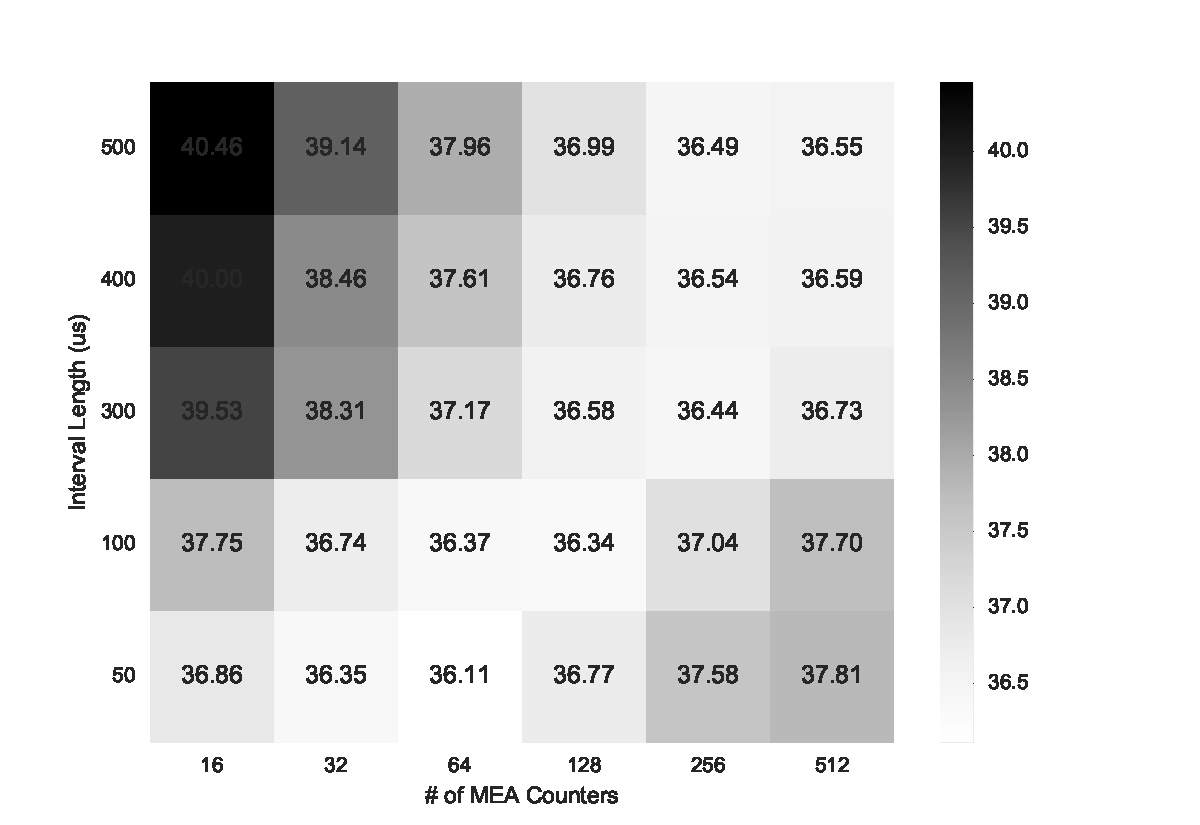
\includegraphics[width=0.46\textwidth]{figures/revised/new/DSE.pdf}
  \caption{Average AMMAT from all workloads under various MemPod configurations.}
  \label{fig:dse}
\end{figure}

Figure \ref{fig:dse} shows our results obtained by taking the average AMMAT from all workloads under each MemPod configuration. Based on the results we derive some observations:

\begin{itemize}
\setlength\itemsep{0em}
	\item MemPod achieves the best performance (lower AMMAT) with 50us intervals and 64 counters per Pod. MemPod's lightweight operation allows for such small intervals. For comparison purposes, HMA \cite{meswani-HPCA21} identified the best epoch length to be 100ms (2000x larger) in order to support all the lengthy processes that take place during a migration event for that method.
	\item The lowest AMMAT values lie on the diagonal of our result matrix.
This implies that the key determinant is the number of migrations, as the
maximum migration rate is (very roughly) a constant across the diagonal.
	\item Few counters and long intervals (inability to react well to
phase changes), at least in this sweep of parameters, appears to be worse than
many counters and small intervals (overly aggressive migration activity).
\ignore{Small intervals with many counters and large intervals with few counters report the largest AMMAT values. We attribute these numbers to each mechanism's ability to adapt to phase changes. Under small intervals it seems beneficial to favor temporal locality since it's more likely we are in the same execution phase after several intervals. Under larger intervals, it's likely that execution is at a different phase between migrations and as such focusing on temporal locality is most likely counter-productive. In this case MemPod needs to identify continuously-used hot pages to increase its odds for successful migrations.

	\item Our results also indicate that each Pod does utilize the higher number of counters and consequently perform more migrations per interval. However all of the evaluated MemPod configurations report degraded performance when the number of counters exceed the optimal (right-hand side of the diagonal in the presented matrix) due to the overhead of migrations. \remark {A.P.: We might want to skip this point}
}
\end{itemize}

The size (in bits) of each counter defines the area requirements of our MEA tracking mechanism. 
\ignore{Based on our observations so far, we expect that smaller intervals would also benefit from smaller counters due to the temporal effects of the counter size variable. We also expect that as interval lengths increase, the optimal counter size will also increase to accommodate the temporal locality trade-off. 
}
Figure \ref{fig:counter_size} presents AMMAT results normalized to a configuration with 2-bit counters as well as the average number of migrations per Pod per epoch (secondary axis). We first observe that 8 bits are sufficient for our workloads, as larger sizes report identical results. We also observe that reducing the counter size to even less than 8 bits benefits performance,
although very marginally.  Small counters, as mentioned, favors recency.
The smaller the interval, the more important recency becomes over accurate
counting; plus, the fewer bits required for accurate counting since there
are fewer events.
Finally, for 50 us intervals, 2 bit counters offer the best performance
(but again, the differences are small).
\ignore{. We see only minor differences in these results,
in large part because of the competing effects of accurate counting (with large counters) and more temporal effects (with small counters). Small counters better capture recency, because fewer divisions are required  \remark{A.P.: Is ``divisions'' the correct word here?} to eliminate a high-access page from the pool and
replace it with a new page.
}

Figure \ref{fig:counter_size_old} shows the same experiment with MemPod's parameters set to 100us intervals and 128 counters. This figure demonstrates that as the interval and number of counters increases (i.e. less focus on temporal locality required), the optimal counter size grows from 2 to 4 bits.

\begin{figure}[h]
	\begin{subfigure}{\linewidth}
    	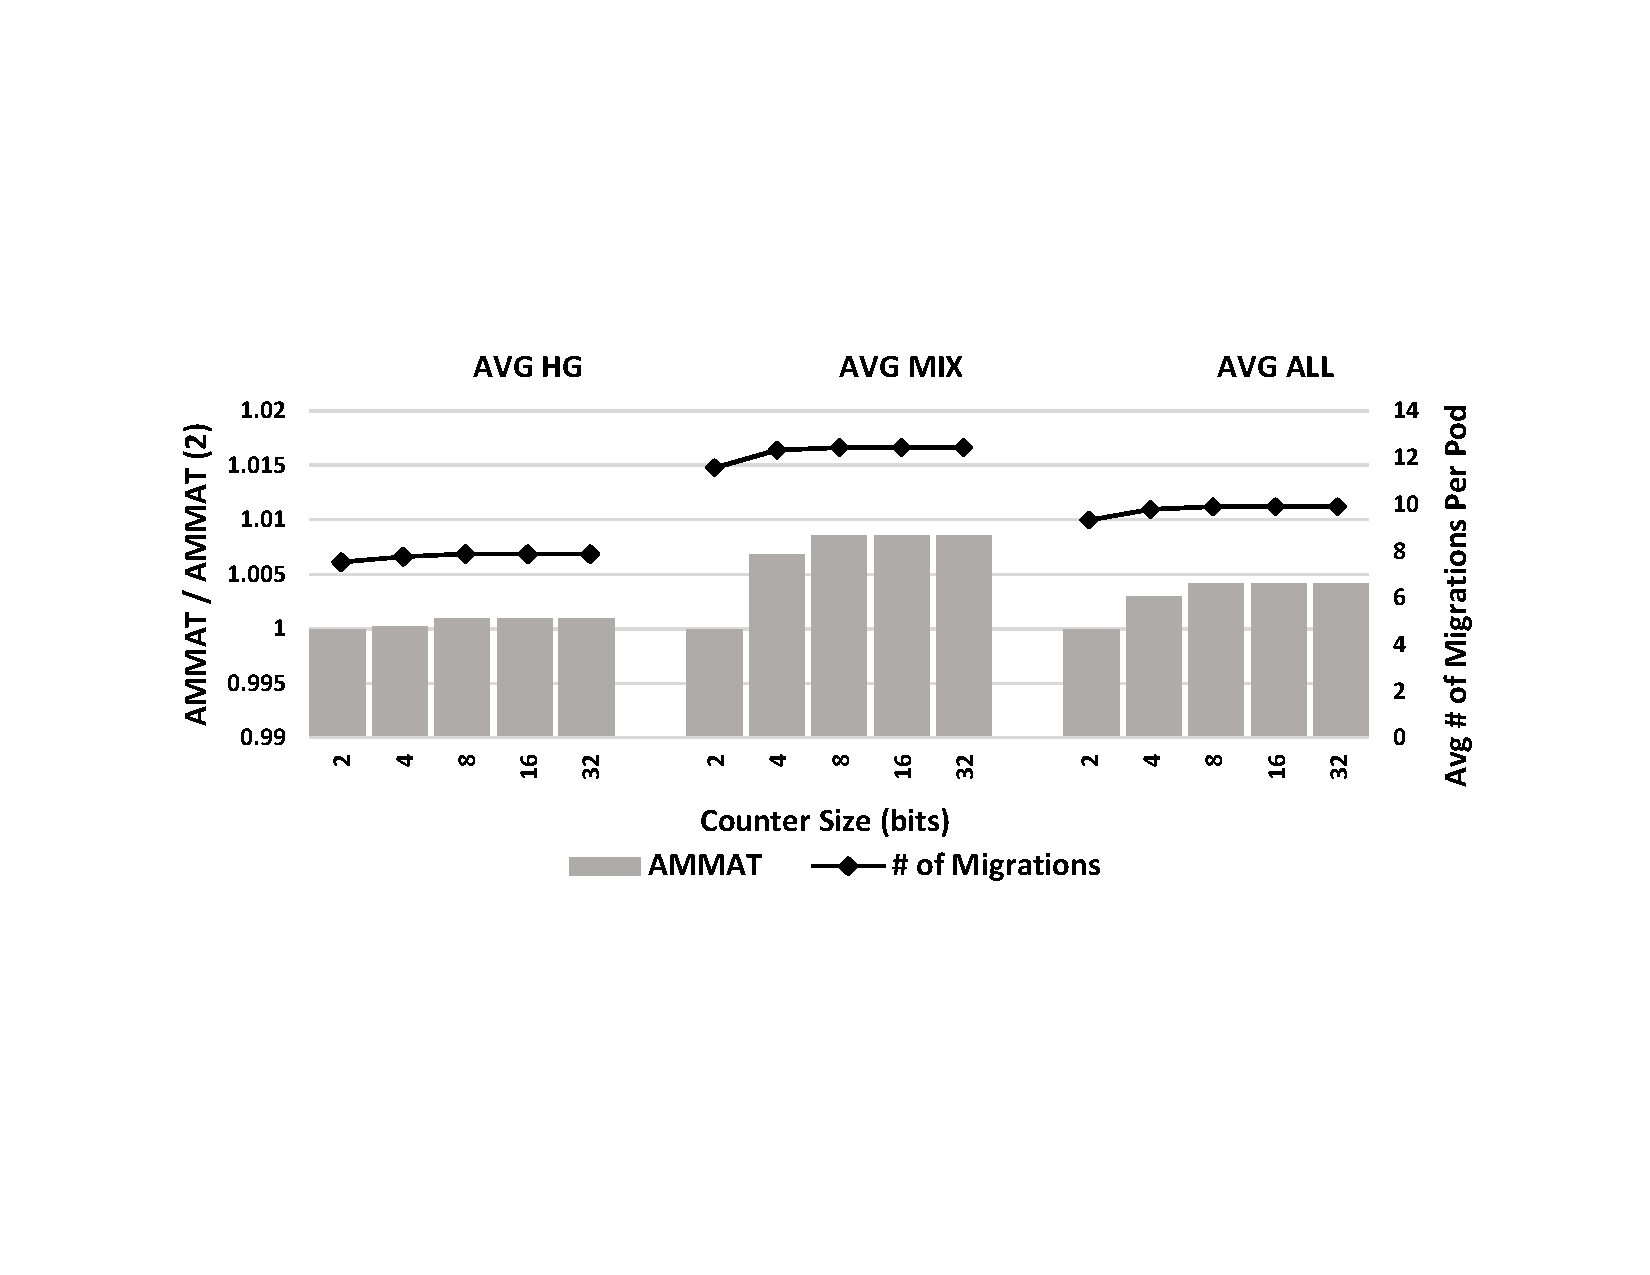
\includegraphics[width=\linewidth]{figures/revised/new/ctr_size.pdf}
    	\caption{MemPod @ 50us, 64 MEA counters \\ \hfill}\label{fig:counter_size}
	\end{subfigure}
	\begin{subfigure}[b]{\linewidth}
    	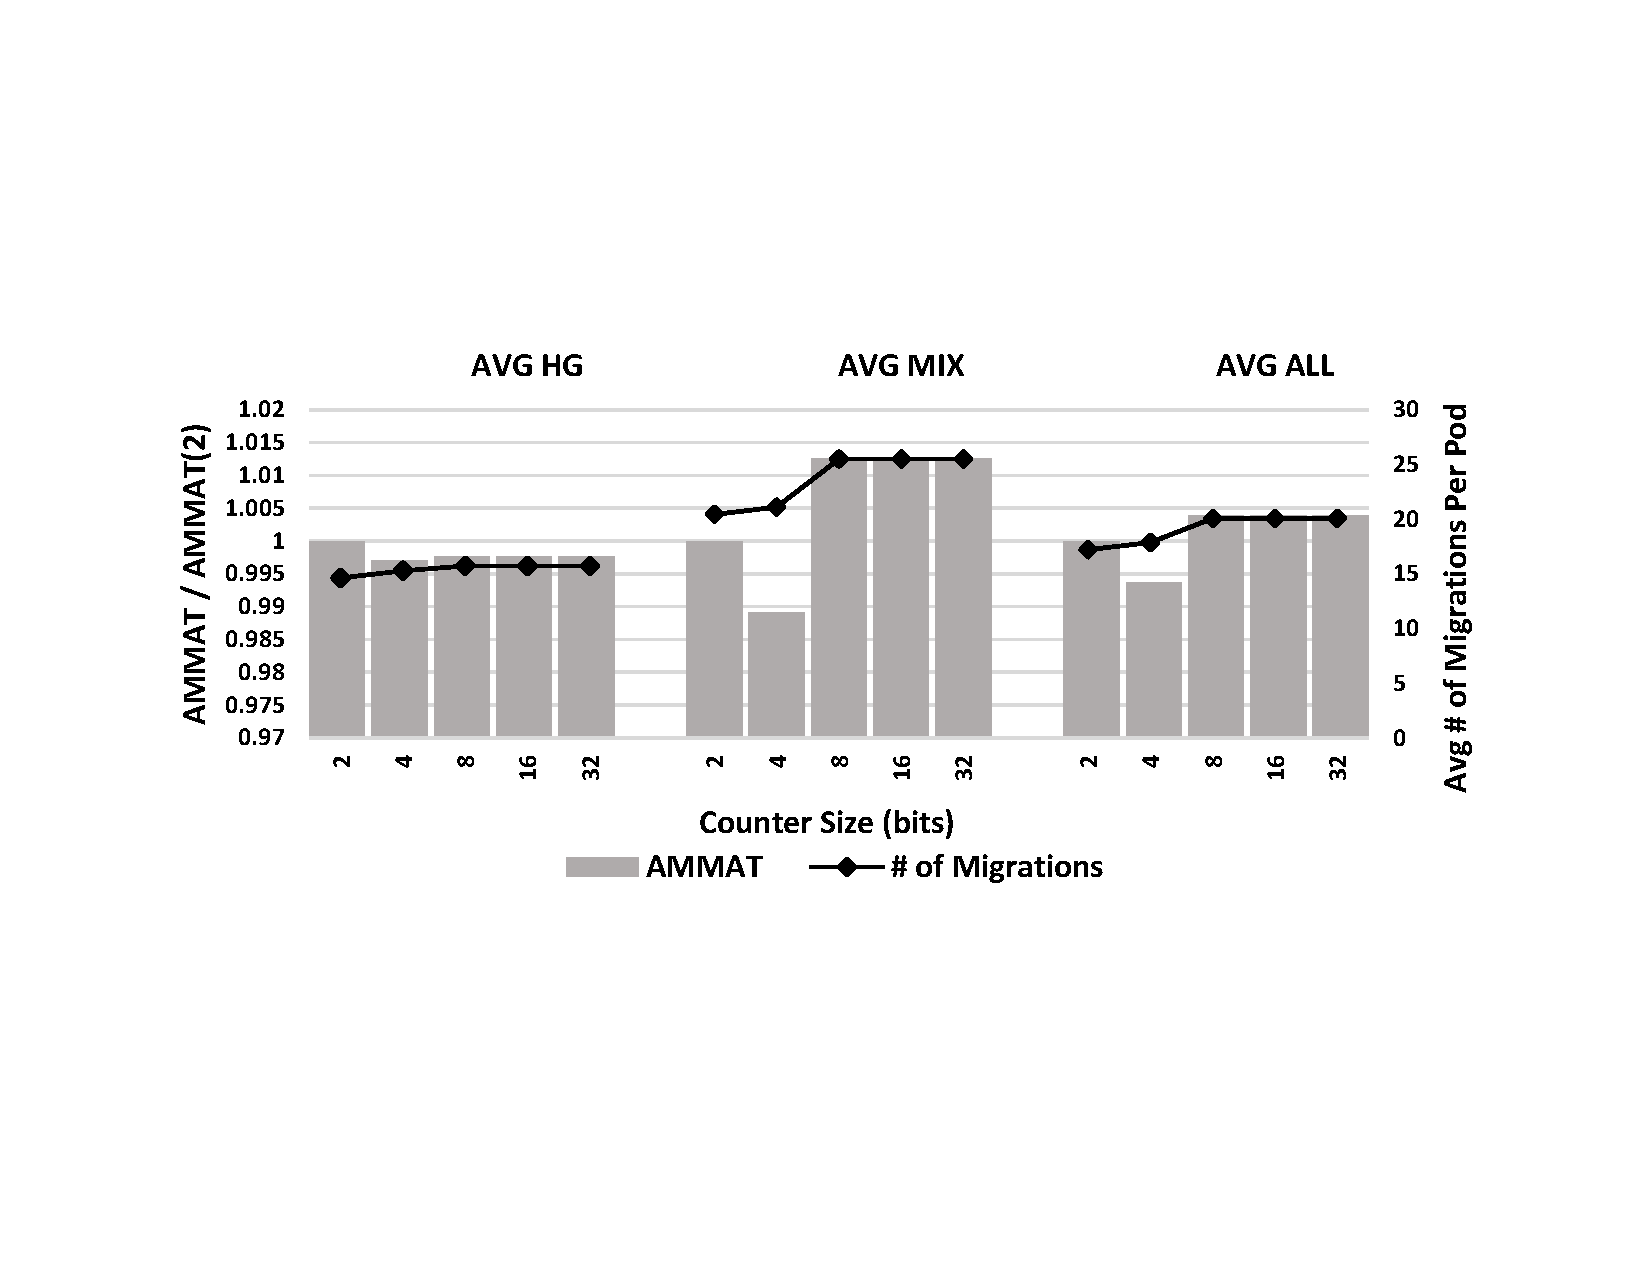
\includegraphics[width=\linewidth]{figures/revised/old/ctr_size.pdf}
    	\caption{MemPod @ 100us, 128 MEA counters}\label{fig:counter_size_old}
	\end{subfigure}
	\caption{Counter size (in bits) Vs Normalized AMMAT (primary axis) and average \# of Migrations per Pod per interval (secondary axis)}
\end{figure}

\begin{figure*}[t]
  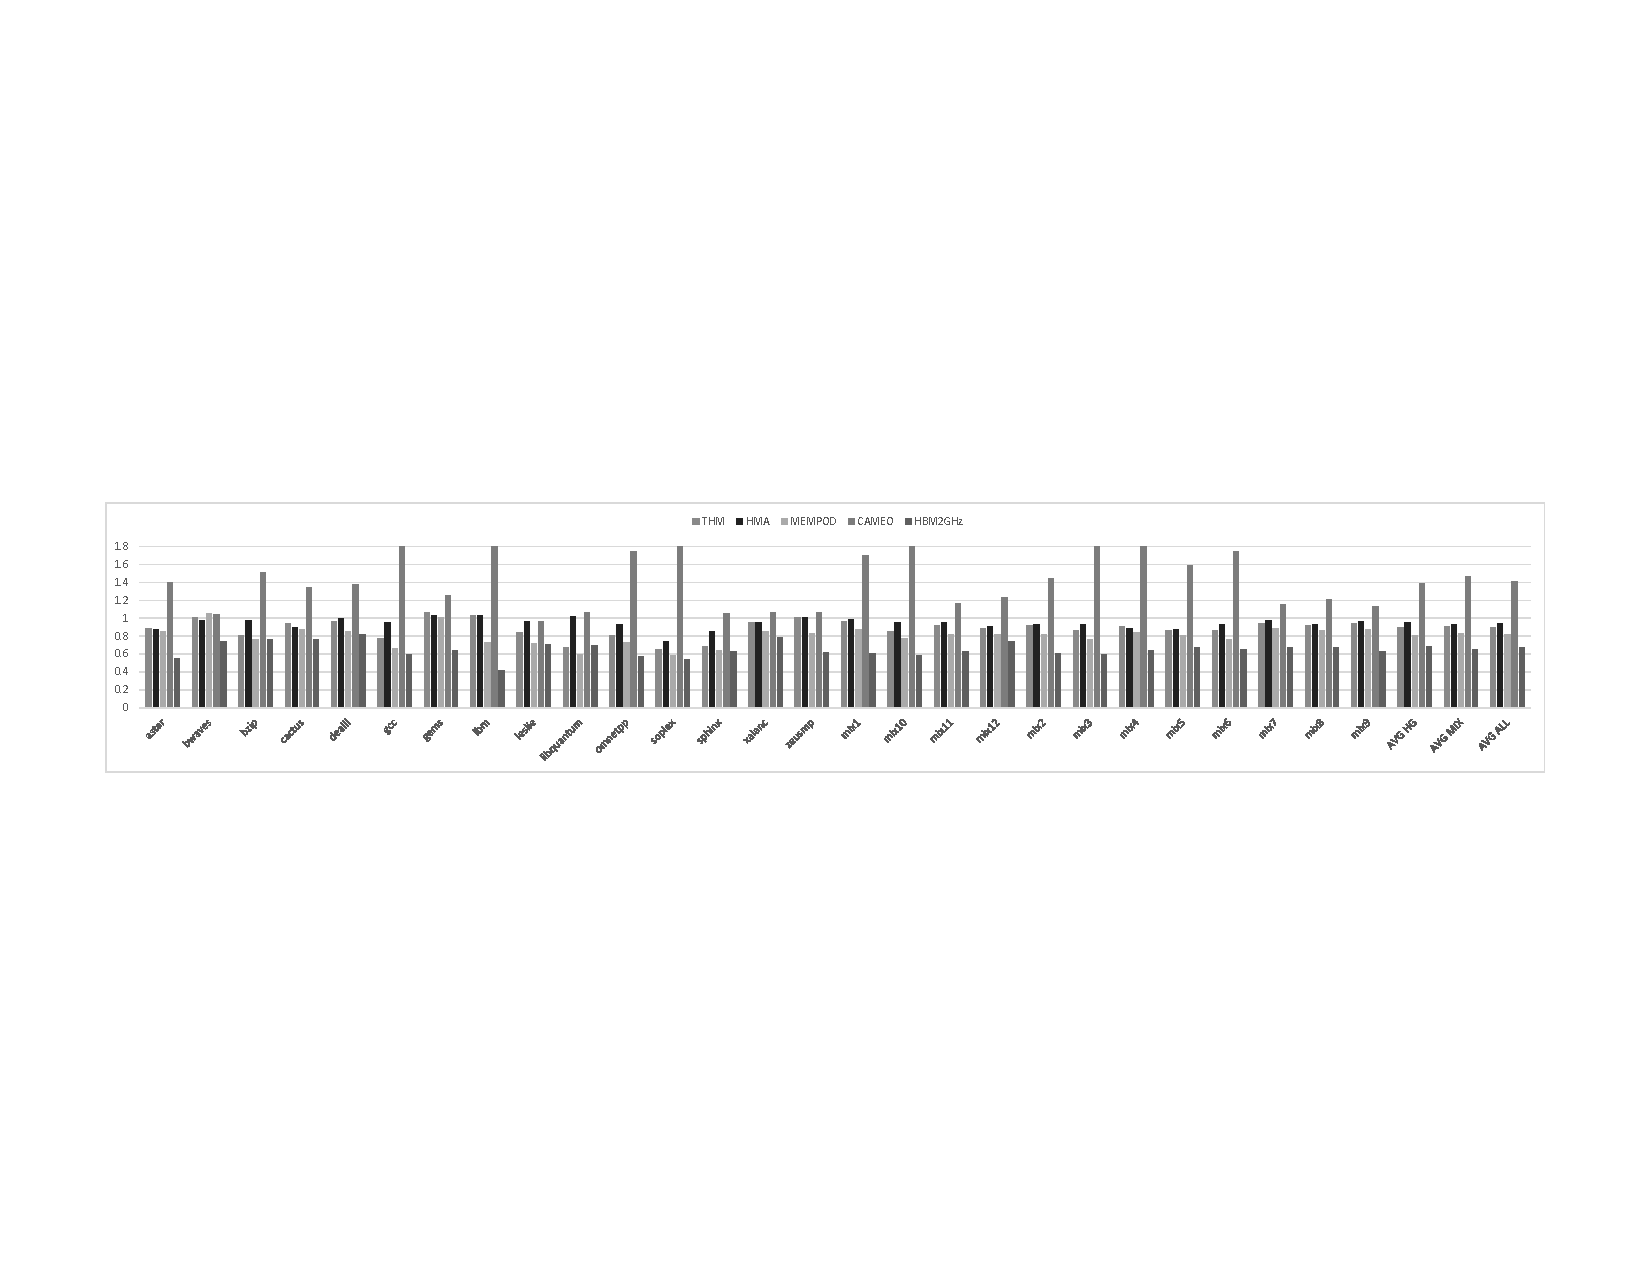
\includegraphics[width=\textwidth]{figures/revised/new/comparison_no_cache.pdf}
  \caption{Performance Comparison: AMMAT is normalized to a hybrid memory without any migration mechanism.}
  \label{fig:performance}
\end{figure*}

Based on these results, we use 64 MEA 2-bit counters over 50us intervals
for subsequent results in this paper.
Each one of the 64 MEA entries needs 21 bits for addressing the 1.1M pages per Pod and 2 bits for its counter, leading to an area cost of only 184B per Pod and 736B total. Compared to the state of the art, MemPod's activity tracking requirement is $\sim$712x smaller than THM's (512KB) and $\sim$13000x smaller than HMA's (9MB).



\subsubsection{Performance Comparison}
\label{sub:performance}

Figure \ref{fig:performance} presents a performance comparison of MemPod, HMA, THM, CAMEO and a configuration with 9GBs of on-chip HBM memory, normalized to the performance of a hybrid memory configuration without migration capabilities. We evaluated all mechanisms with migration-related caching disabled. 

In order to model HMA's penalties more accurately, we profiled sorting 4.5M integers using quicksort ( NlogN complexity) on a real system with a recent Intel Core i7 processor running at 2.1GHz. Our experiment showed that sorting all of HMA's activity tracking counters, at these memory sizes, takes 1.95s on 
average. When we scale this overhead to our simulated 3.2GHz core, the expected delay would be approximately 1.2s, which is much larger than the proposed optimal interval size for HMA. We instead assumed a very generously reduced overhead of 7ms per interval, assuming we could sort in parallel and discard obvious low values before sorting.

\ignore{In our following experiments we assume a highly optimized sorting technique for HMA and we add a fixed penalty of 5 processor cycles per counter (7ms total sorting overhead per interval).
}

Based on the results we make the following observations:
\begin{itemize}
\setlength\itemsep{0em}
	\item MemPod outperforms the state-of-the-art competitors in the majority of our workloads, and in several cases is very close to an HBM-only 
configuration. MemPod improves AMMAT over a two-level memory 
without migrations by 19\% on average.
	\item On average, CAMEO reports AMMAT degradation of 41\% over the no-migration scheme. The negative impact is caused by our high ratio of
slow to fast memory capacity.  Given CAMEO's algorithm, 9 slow lines
compete for one fast line.  At that ratio, it is much more likely for
two or more lines to thrash competing for the one spot.
From our experiments, we observe CAMEO to force the most movement despite the
fact that each move ismuch smaller.  CAMEO moves 3.9GB of data on average per 
8-core experiment. For comparison purposes, MemPod moved 3.1GB on average, however migration traffic was divided between Pods, resulting in 804MB per Pod. 
THM moved 865MB on average and HMA moved 578MB due to its large intervals. 
We also frequently observed frequent wasted migrations with CAMEO, where a 
line is 
evicted before it is touched. 
\ignore{Optimizations such as intelligent line allocation to segments can significantly improve CAMEO's performance and reduce intra-segment conflicts, however to maintain a fair evaluation, CAMEO is evaluated under the same memory organization as the rest of the mechanisms.\remark {A.P.: Should we make this a subsection on its own?}
}
	\item On average MemPod reports 21\% higher AMMAT than HBM-only, while THM and HMA report 33\% and 40\% respectively.
	
	\item In some workloads migration overall is harmful to performance, 
as observed with the bwaves workload, where a no-migration scheme reports 
higher performance (lower AMMAT). We observe that in those cases, MemPod leads to deteriorated performance compared to the other mechanisms. However, in the cases of lbm and zeusmp, 
MemPod increases performance, while THM, HMA and CAMEO report higher AMMAT than the no-migration scheme.

	\item HMA and MemPod outperform HBM-only when executing the libquantum experiment. In the case of libquantum, the working set size fits entirely in our fast memory. As a result, after some migrations, the entire working set will be present in HBM.  With an HBM-only system and no migrations, pages
are inserted sequentially by address.  In a migration-based system, 
simultaneously-hot pages are inserted together after each epoch.  As the
DRAM row buffer is bigger than a page, we find that the co-location of
simultaneously-hot pages increases row buffer hit rate from 7\% (HBM only)
to 90\% (MemPod), with 87\% of those taking place in fast memory.  HMA also sees an improvement in row buffer hit rate. THM and CAMEO cannot take advantage of the small footprint due to their restricted migration flexibility (only one hot page/line per segment can reside in fast memory).
\remark{Don't know how to explain THM, but the effect is smaller -- what is
the row buffer hit rate?\\A.P.: THM's results were wrong. The updated results and graph show that it doesn't outperform HBM.}
%However, correct timing is the driving factor behind this impressive performance increase. Our results show the row-buffer hit ratio to be \TODO{??x} times higher than the HBM-only memory system (and random page assignment). Apparently, page migrations resulted in an in-HBM page order that increases page hits and exploits a much higher degree of memory parallelism from the application. This result could be further explored and intentionally recreated in some future work.
\end{itemize}

\subsubsection{Caching Effect}
\ignore{
\begin{figure}
  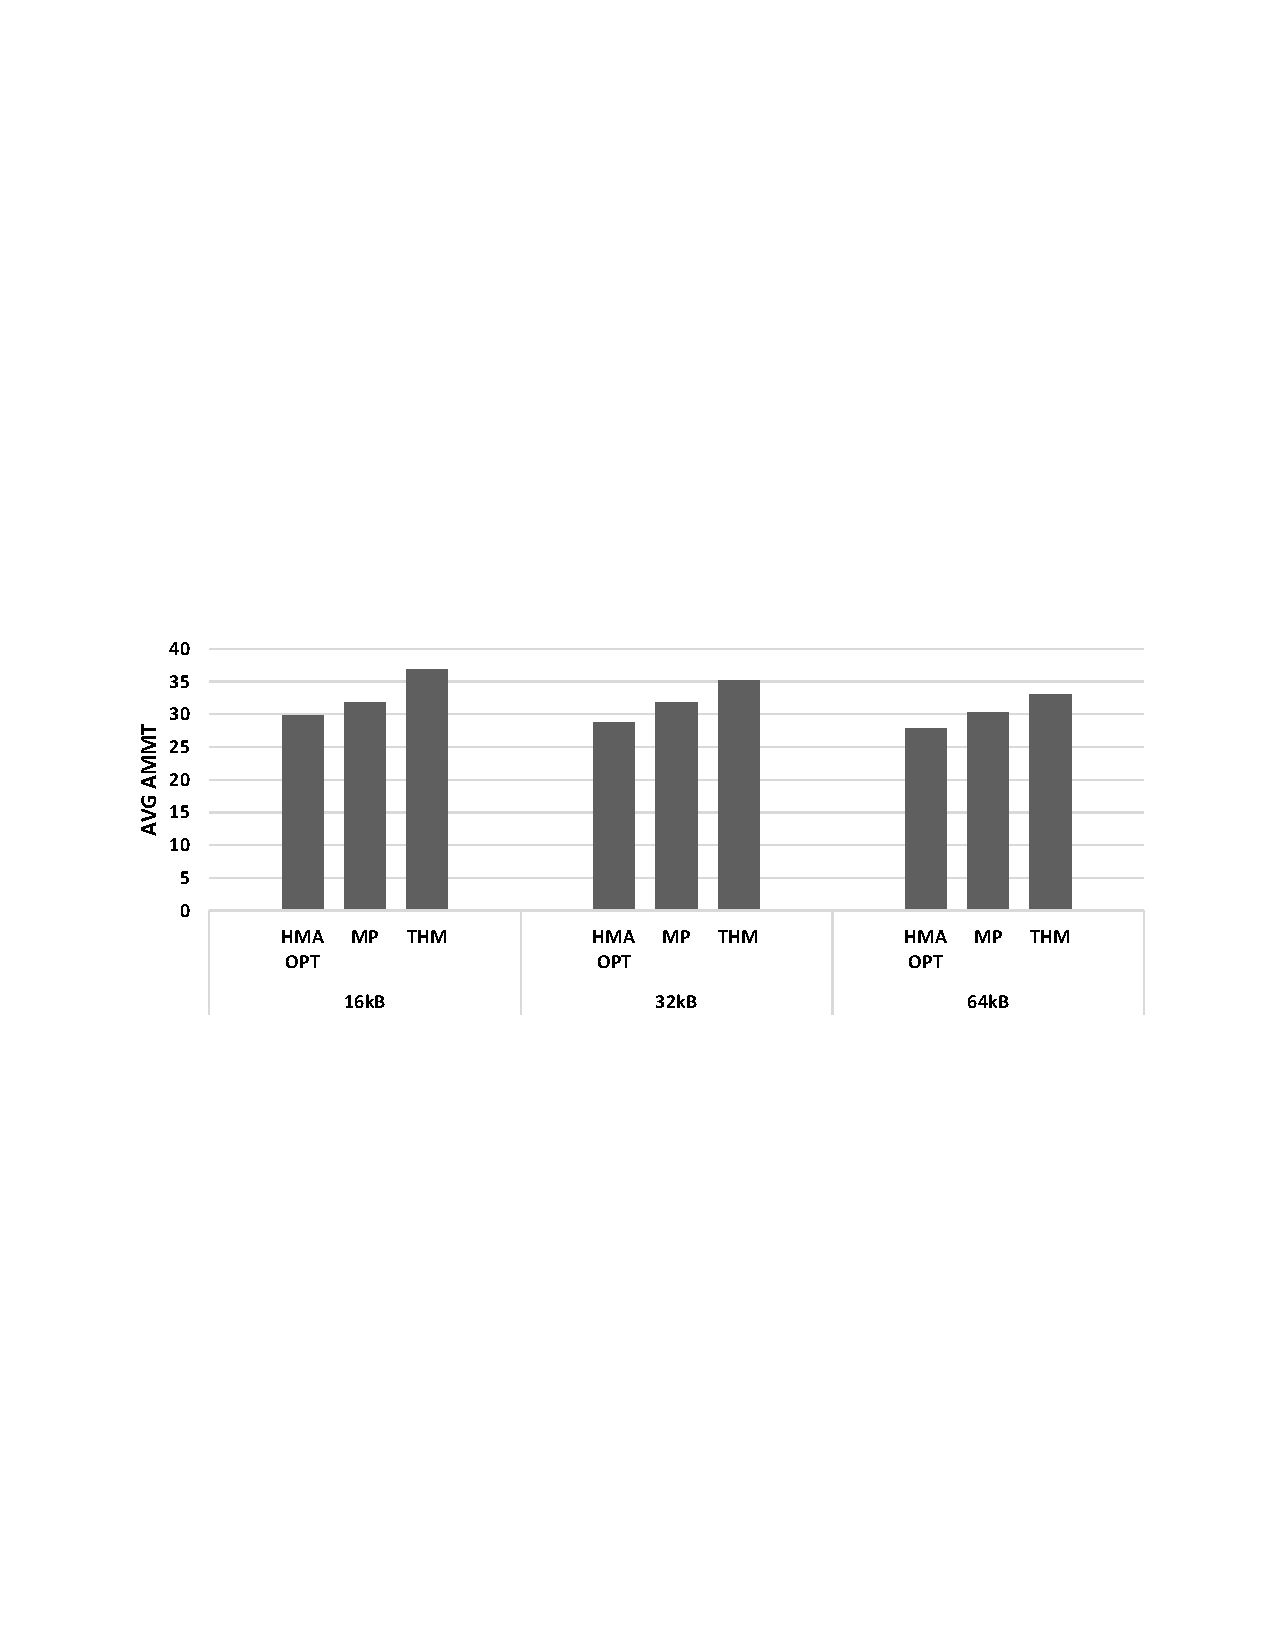
\includegraphics[width=0.46\textwidth]{figures/cache_impact.pdf}
  \caption{Cache Impact. AMMAT normalized to stock TLM (no migrations)}
  \label{fig:cache}
\end{figure}

\remark{A.P.: I don't have CAMEO results with caching yet. Not sure if it will be ready on time but I'm working on it.}

\remark{A.P.: Need to change the structure of this section due to issues with results.}


Migration mechanisms will be forced to include a cache as activity tracking and remap table structures are too large to store on-chip. The use of a cache will unavoidably hinder performance. In this experiment we evaluate the impact of a cache on each mechanism's performance. As described in Section \ref{sec:Architecture}, each mechanism has different cache requirements. THM caches its counters and remap table together with its SRT structure. HMA has no need for a remap table but has high storage requirements for its counting mechanism. MemPod must cache only its remap table as MEA counters will be on chip. We simulated each mechanism with 16, 32 and 64 KB of cache. For MemPod, the available cache capacity was divided equally over four Pods. All mechanisms use the stacked memory as backing store for their tracking information.

HMA's design further complicates this study, as sorting all activity counters at each epoch is performed by the OS, utilizing the cpu's cache instead of the dedicated migration cache. In our results, we present ``HMA-OPT'', an HMA flavor that does not take into account any penalties for OS interrupts, TLB shootdowns, Page Table (PT) updates, walks and misses, or sorting of the large
pool of counters.
We also do not model the application-level effects of starting with a cold TLB after each interval, which only affects HMA.

Figure \ref{fig:cache} shows our results obtained by taking the average AMMAT from all our workloads for each mechanism. HMA-OPT reports the lowest AMMAT, albeit unrealistic and MemPod outperforms every other mechanism regardless of the cache size. MemPod outperforms THM by 9\% with a 64kB cache, while HMA-OPT outperforms MemPod by 9\%.
}

Migration mechanisms will be forced to include a cache as activity tracking and remap table structures are too large to store on-chip. The use of a cache will unavoidably hinder performance. Each mechanism has different cache requirements. THM caches its counters and remap table together with its SRT structure. HMA has no need for a remap table but has high storage requirements for its counting mechanism. MemPod must cache only its remap table as MEA counters will be on chip. 

In this experiment we evaluate the impact of a cache on MemPod's performance and we also compare it against HMA and THM when operating with a cache. MemPod was configured with the optimal parameter values identified over the course of this section. Every mechanism was evaluated with 16, 32 and 64 KB of cache. For MemPod, the cache capacity is distributed equally over its four Pods. A part of stacked memory was partitioned to serve as each mechanism's backing store.

In our implementation, each cache miss injects a read request to retrieve missing data. Since all of MemPod's cache misses will occur due to Remap Table updates or lookups it becomes a blocking request for the affected page. All incoming requests to that page need to be delayed until the missing data is retrieved. In-flight requests are not affected by incoming cache misses.

%\ignore{
%\begin{figure}[h]
%	\begin{subfigure}{\linewidth}
%    	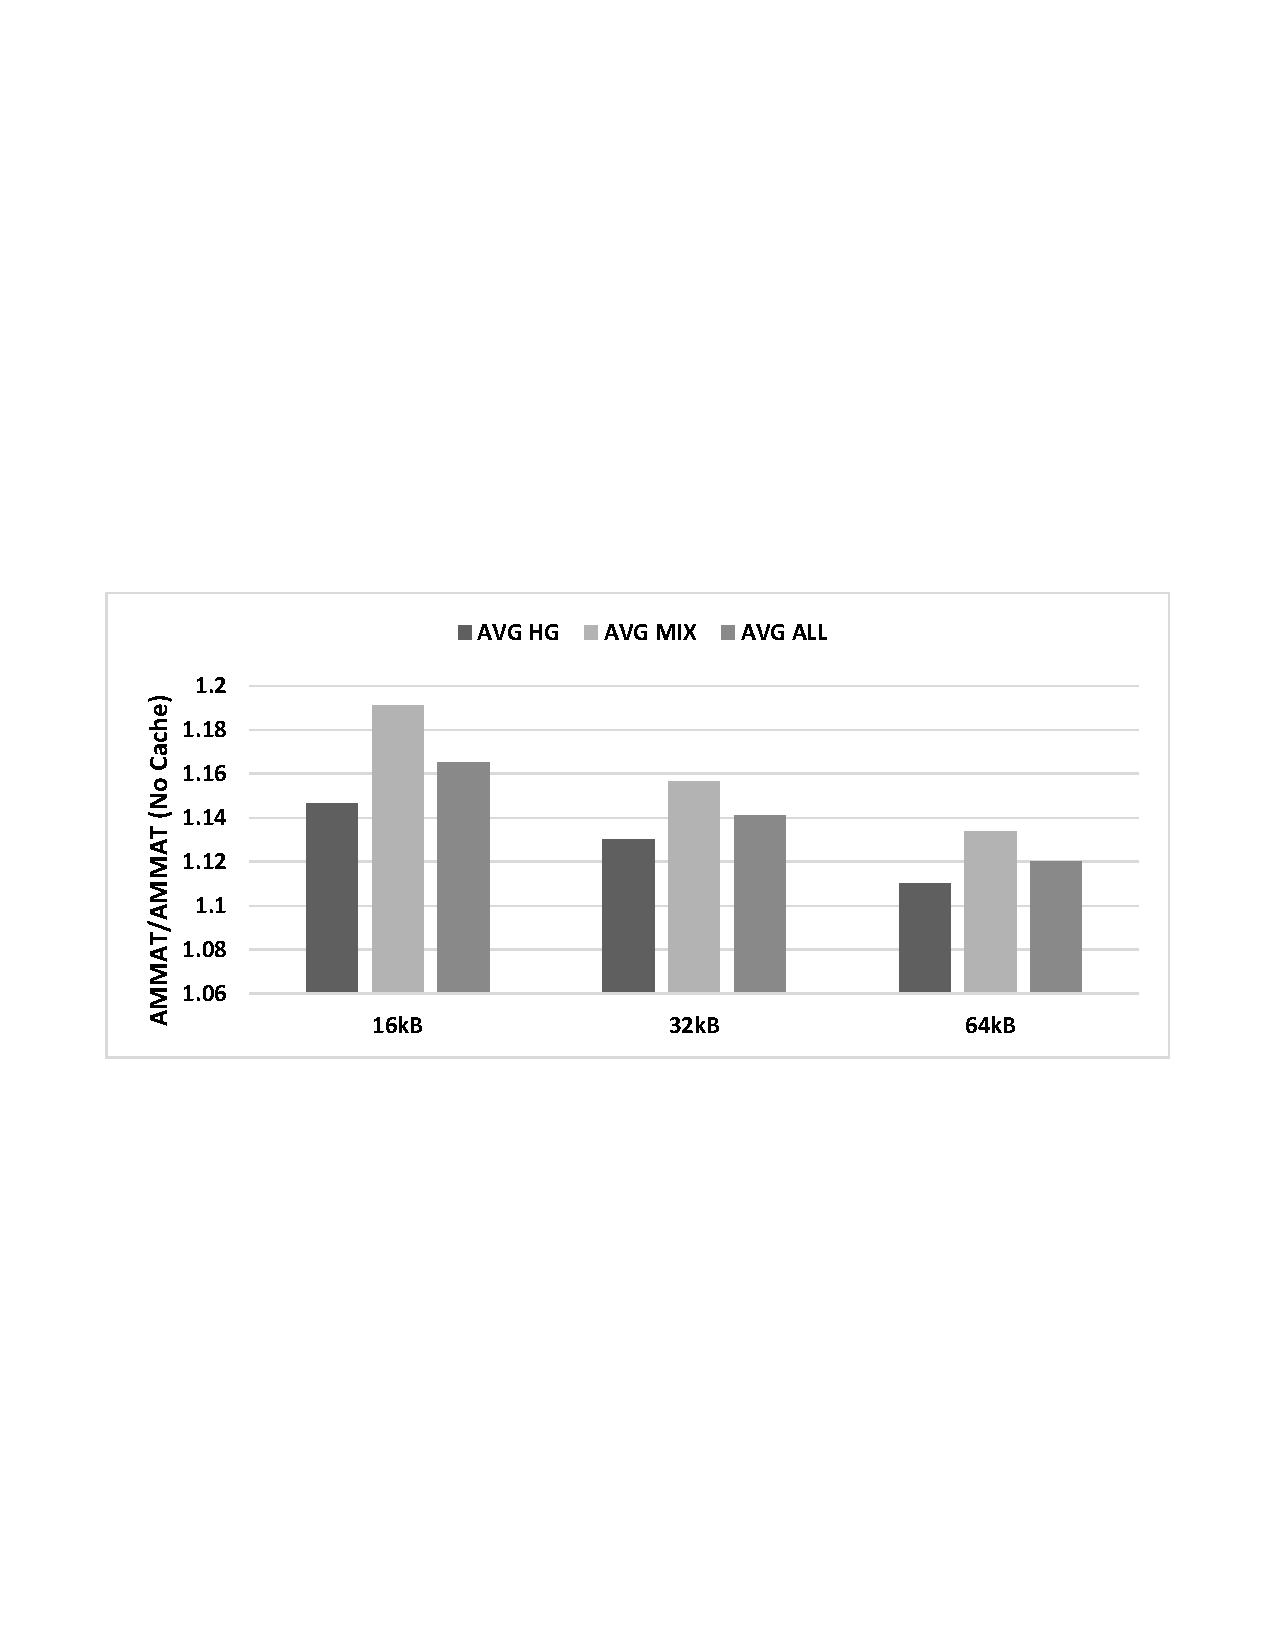
\includegraphics[width=\linewidth]{figures/revised/new/cache_impact.pdf}
%    	\caption{AMMAT normalized to each mechanism w/o caching \\ \hfill}\label{fig:cache_impact}
%	\end{subfigure}
%	\begin{subfigure}[b]{\linewidth}
%    	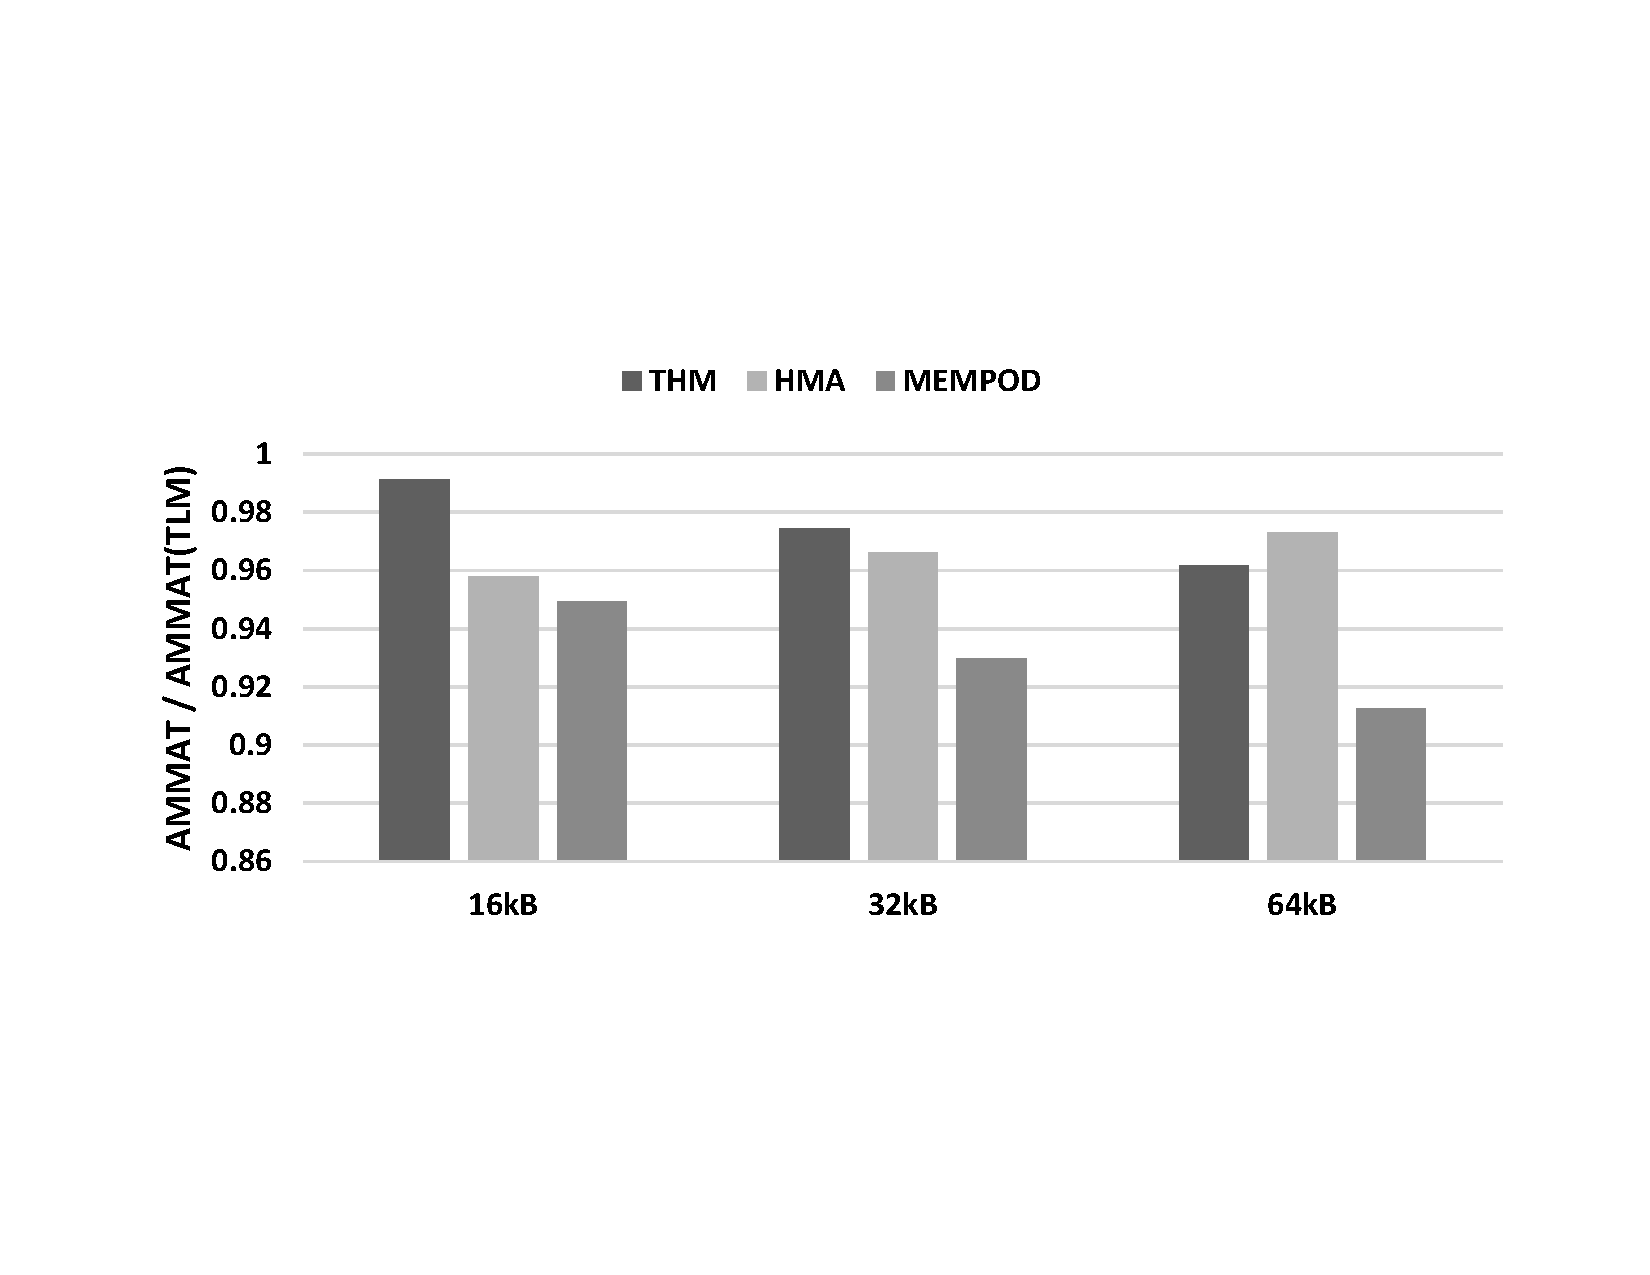
\includegraphics[width=\linewidth]{figures/revised/new/cache_norm_tlm.pdf}
%    	\caption{AMMAT normalized to stock TLM (no migrations)}\label{fig:cache_norm_tlm}
%	\end{subfigure}
%	\caption{Sensitivity Analysis: Cache Size}
%\end{figure}
%}

\begin{figure}[h]
  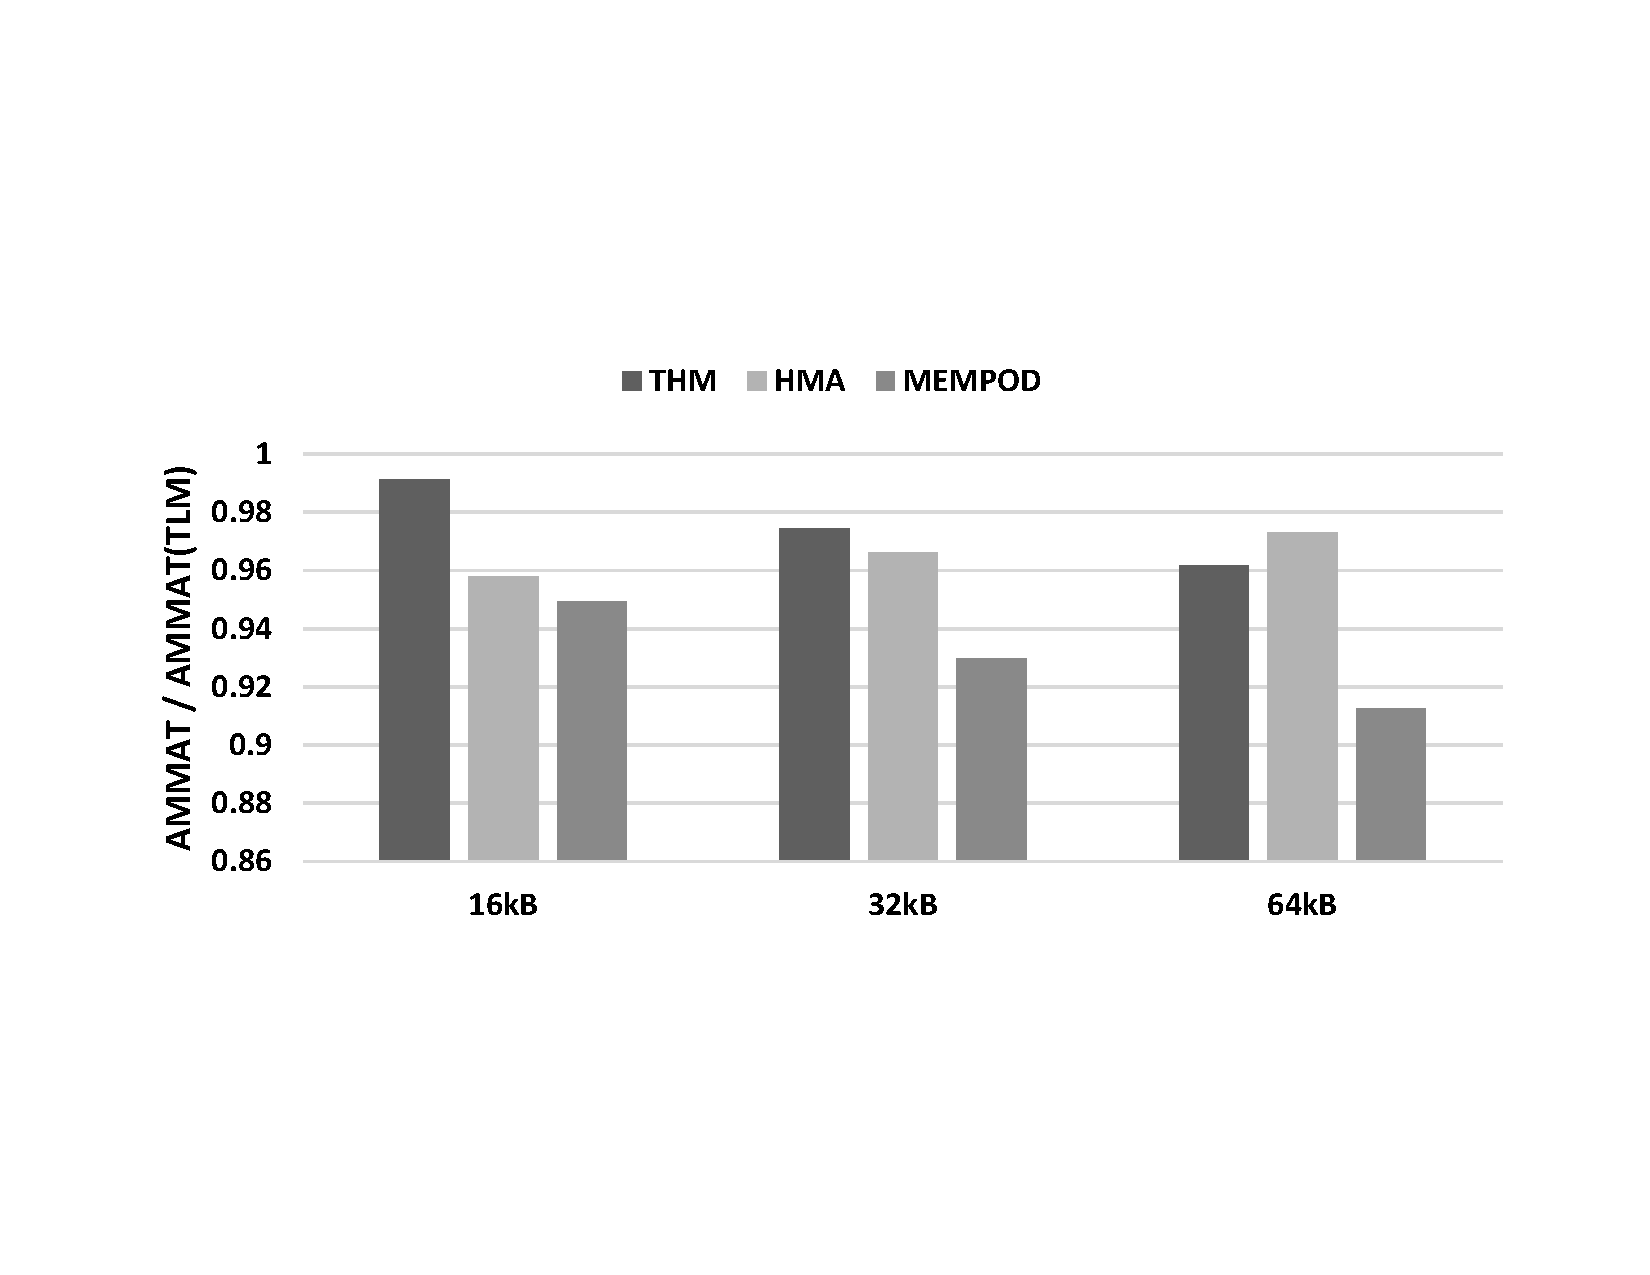
\includegraphics[width=0.46\textwidth]{figures/revised/new/cache_norm_tlm.pdf}
  \caption{Scalability to faster memories. AMMAT normalized to a DDR4-only memory.}
  \label{fig:cache_norm_tlm}
\end{figure}

Figure \ref{fig:cache_norm_tlm} shows our results obtained by taking the average AMMAT from all our workloads for each cache size for each mechanism. We present AMMAT results normalized to a two-level memory configuration without any migration mechanism. With 16, 32 and 64kB of cache, MemPod reports 4, 7 and 9\% AMMAT improvement over TLM and outperforms the other mechanisms.

For 16, 32 and 64kB of cache, the impact on MemPod's performance (when compared to its performance without a cache) is 16, 14 and 12\% respectively. THM reports impacts of 12, 10 and 9\%. Interestingly, HMA reports lower performance impact with smaller cache sizes rather than larger. Our investigation revealed that the extra cache misses caused by a smaller cache lead to a reduced number of incoming requests to be serviced per interval. As a result, HMA's activity tracking counters have lower values at the end of the interval, leading to fewer migrations. As demonstrated earlier in Section \ref{sec:MEA}, HMA (using Full Counters) has a low prediction accuracy. As such, by reducing the number of migrations, we observe the number of requests serviced by the fast memory to 
increase, due to hot pages that were not replaced as aggressively.

\subsubsection{Scalability}

MemPod is designed to be scalable with future technology.  If we grow memory
sizes by increasing the number of pods, the size of the remap table and the 
size of the MEA counters will remain constant (per pod, and thus per memory
page) if the memory per pod remains constant.  If instead we increase
memory capacity per pod, the size of the remap table (per memory page)
will go up only with the log of the per-pod memory. If we choose to scale
the number of counters with the size of memory per pod, it will go up
similarly; however, if we do not scale up the counters at the same rate
(e.g., four times the memory, but double the counters), then the cost
of the counters (per memory page) will go down.

Additionally, the memory traffic caused by migrations will remain distributed
and off the primary processor interconnect.

We also expect the latency differential between main memory levels to 
continue to grow.  This will happen as 3D memory parts mature, and as
we integrate new memory technologies into the system (e.g. hybrid
volatile and non-volatile memory systems).
To examine this, we model a system where both the 3D DRAM and the DDR memory
are faster, but the 3D DRAM is accelerated further resulting in a higher
latency ratio between the two. 
In particular, we simulate a 4GHz HBM as our stacked memory and a DDR4-2400 as our off-chip memory. Since we are modelling a future system, we reduced the fixed penalty for HMA's sorting process from 7ms to 4.2ms (40\% reduction) in order to model future faster processors.
We assume no cacheing effects in this experiment.

\begin{figure}[h]
  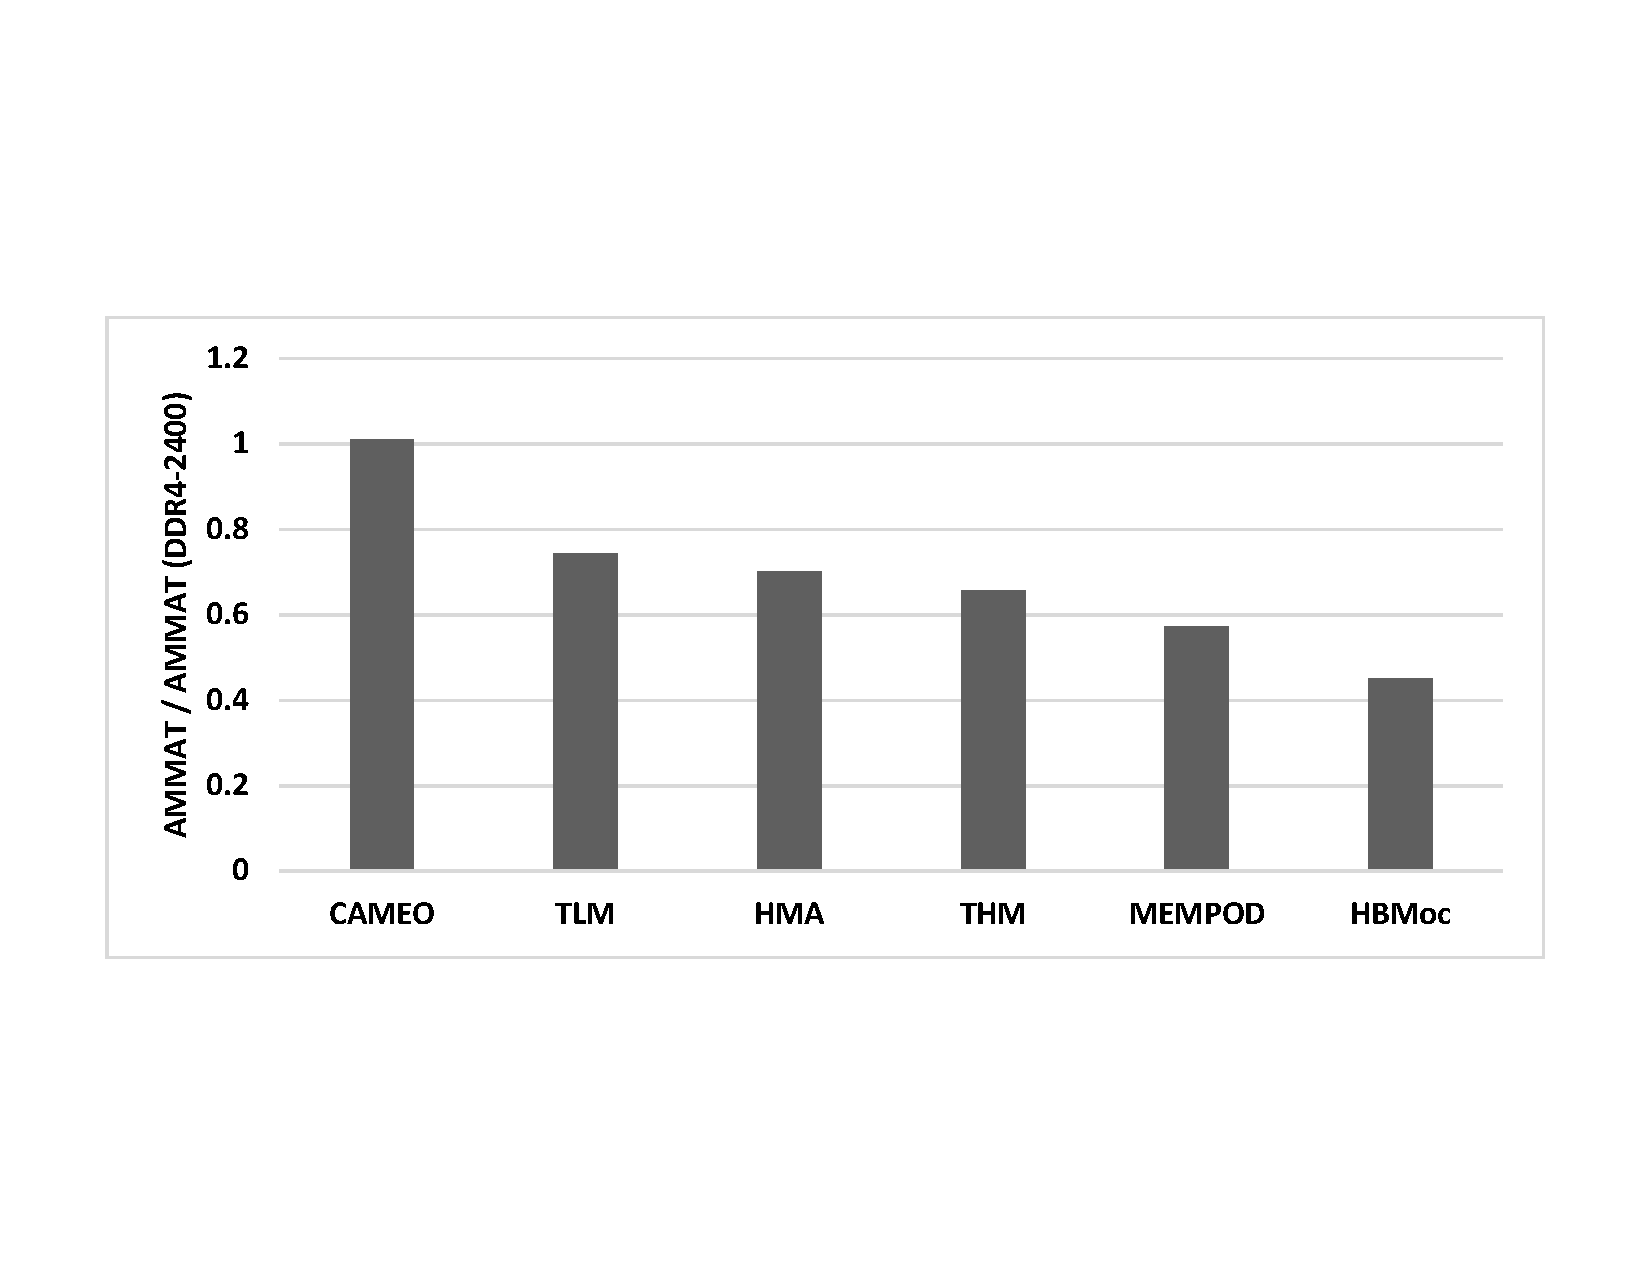
\includegraphics[width=0.46\textwidth]{figures/revised/new/scalability_speed.pdf}
  \caption{Scalability to faster memories. AMMAT normalized to a DDR4-only memory.}
  \label{fig:scalability}
\end{figure}

Figure \ref{fig:scalability} shows our AMMAT results, normalized to a configuration with 9GBs of off-chip DDR4-2400. The label ``HBMoc'' shows a 9GB configuration with overclocked HBM only. We first observe that CAMEO now reports a 1\% AMMAT degradation. The increase in speed differential between stacked and off-chip memory appears to be beneficial for CAMEO, however we can still observe the impacts of intra-segment conflicts. Compared to a configuration with no migration support (TLM), HMA improves AMMAT by 2\%, THM by 13\% and MemPod by 24\%. The overclocked HBM-only configuration is 40\% faster compared to TLM.

